O Quick Sort é uma técnica de ordenação que utiliza a estratégia de divisão e conquista. Essa abordagem consiste em reorganizar a lista de tal maneira que os elementos menores que um elemento selecionado, chamado pivô, fiquem à sua esquerda, enquanto os maiores ficam à direita. Este processo é realizado de maneira recursiva, diminuindo progressivamente o tamanho das listas a serem ordenadas\cite{devto_quick_sort}.

Os passos fundamentais são:

1- Seleção do Pivô: Um elemento da lista é escolhido para ser o pivô.
2- Particionamento: A lista é reorganizada de forma que todos os elementos à esquerda do pivô sejam menores que ele, e todos à direita sejam maiores. Após essa etapa, o pivô estará em sua posição definitiva, resultando em duas sublistas não ordenadas. Esta etapa é crucial para o processo.
3- Ordenação Recursiva: As sublistas contendo os elementos menores e maiores que o pivô são ordenadas recursivamente.
4- Caso Base: A recursão tem como caso base listas de tamanho zero ou um, que naturalmente estão ordenadas. O algoritmo termina quando todas as sublistas alcançam esse estado.

A eficiência do Quick Sort é significativamente influenciada pela escolha do pivô e pela implementação do processo de particionamento. Diferentes métodos para estas etapas podem resultar em variações substanciais no desempenho do algoritmo, especialmente em diferentes tipos de conjuntos de dados. Neste trabalho iremos fazer testes com 4 tipos diferentes de pivô: 
Versão 1: Pivô como primeiro elemento.
\begin{figure}[H]
    \centering
    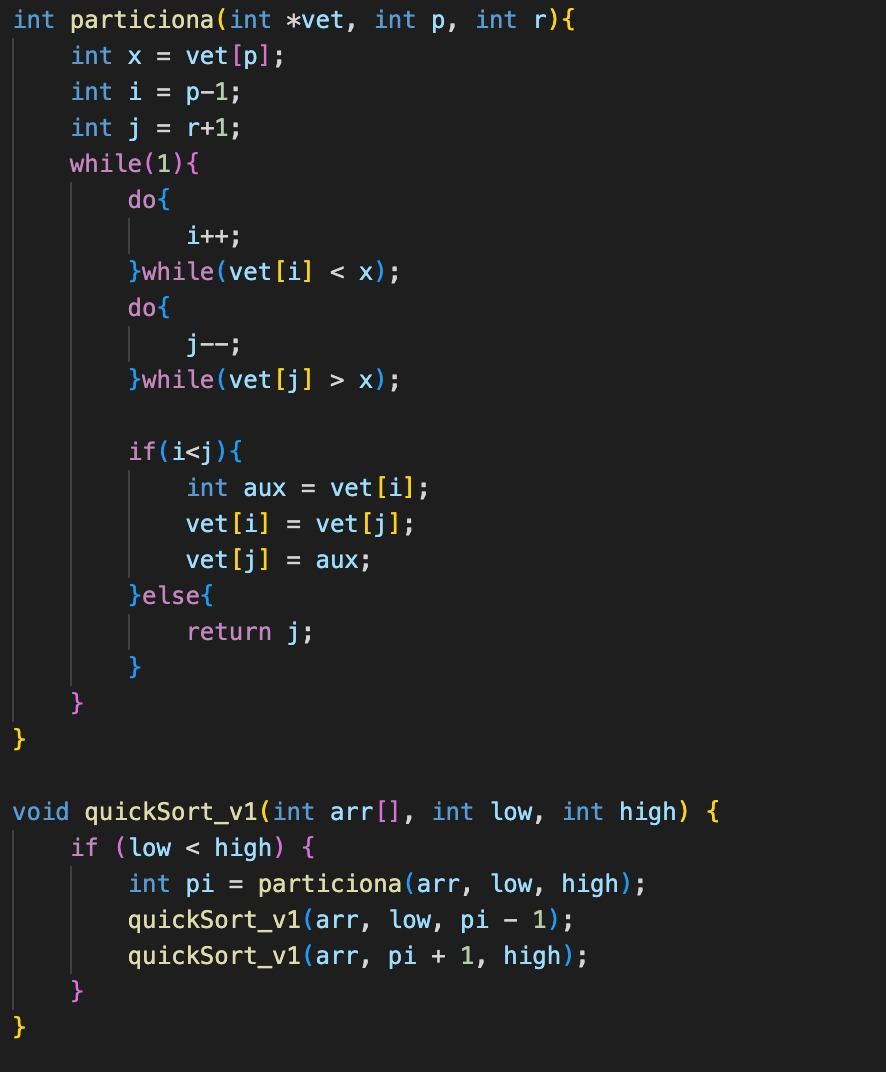
\includegraphics[width = 10cm]{Imagens/Quick Sort/quick1.jpeg}
    \caption{Quick Sort 1}
    \label{grafico_insert}
\end{figure}
Esta é a versão clássica do Quick Sort, onde o primeiro elemento do segmento do array que está sendo ordenado é escolhido como pivô. O objetivo do pivô é ajudar na divisão do array em duas partes, onde um lado contém elementos menores que o pivô e o outro lado contém elementos maiores. Esta versão é simples e eficaz, mas pode ter desempenho subótimo em arrays já ordenados ou quase ordenados.
Versão 2: Pivô como média dos elementos.
\begin{figure}[H]
    \centering
    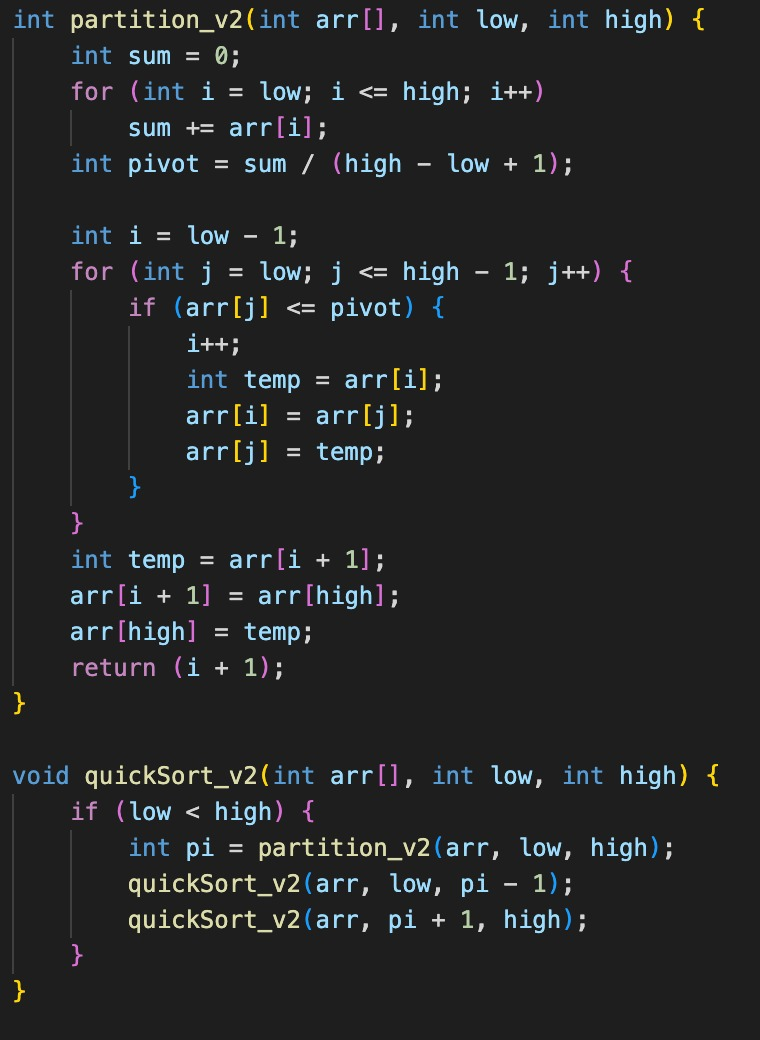
\includegraphics[width = 10cm]{Imagens/Quick Sort/quick2.jpeg}
    \caption{Quick Sort 2}
    \label{grafico_insert}
\end{figure}
Nesta versão, o pivô é escolhido como a média dos valores do segmento do array a ser ordenado. Ao usar a média, busca-se um valor de pivô mais representativo do conjunto de dados, o que pode resultar em uma divisão mais equilibrada do array, especialmente em casos onde os dados têm uma distribuição mais uniforme. Esta abordagem pode melhorar o desempenho em comparação com a escolha do primeiro elemento como pivô.
Versão 3: Pivô como mediana de três elementos.
\begin{figure}[H]
    \centering
    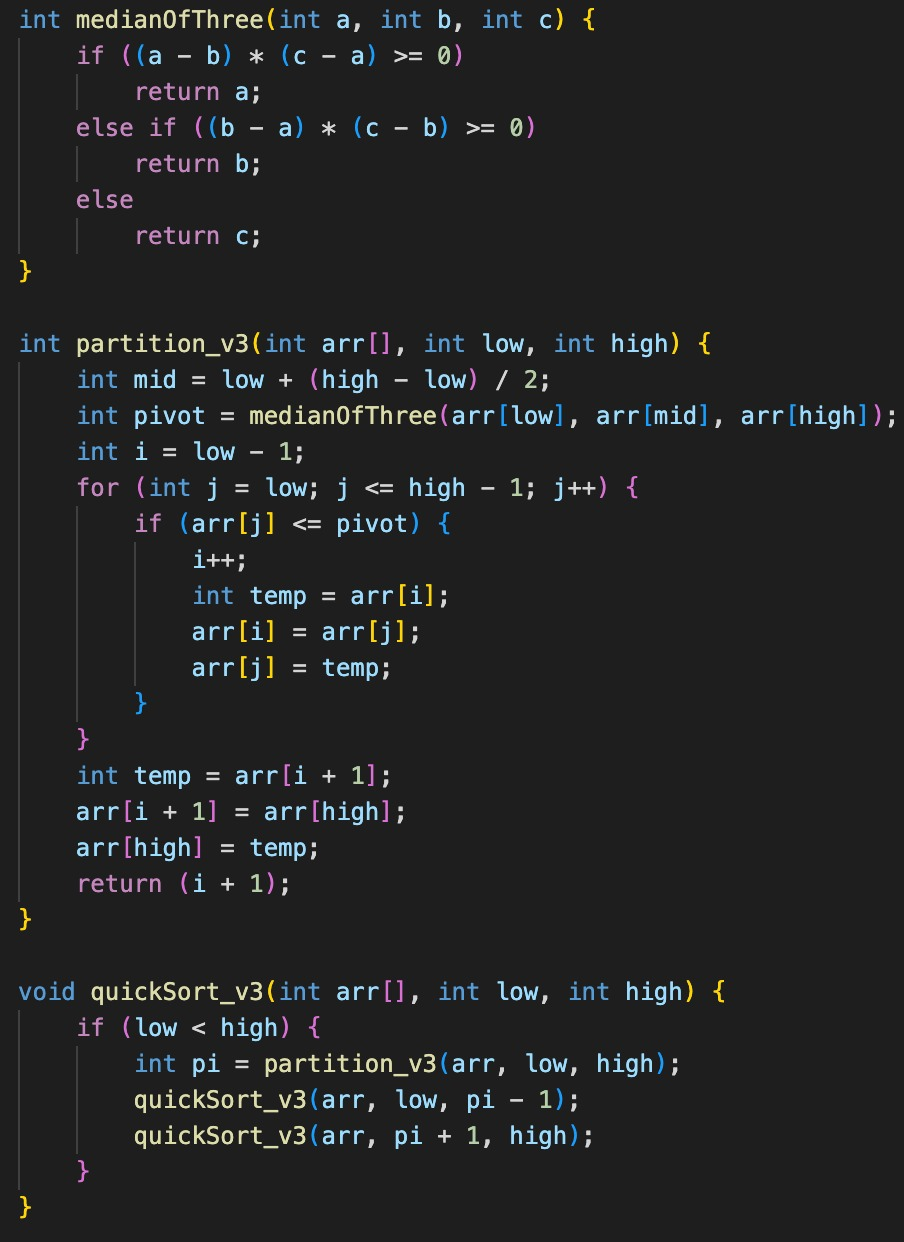
\includegraphics[width = 10cm]{Imagens/Quick Sort/quick3.jpeg}
    \caption{Quick Sort 3}
    \label{grafico_insert}
\end{figure}
Aqui, o pivô é escolhido como a mediana de três elementos selecionados: o primeiro, o último e o elemento do meio do segmento do array. Esta estratégia é uma tentativa de encontrar um bom pivô que seja mais representativo do array inteiro, reduzindo a chance de pior caso (como em arrays já ordenados). Escolher a mediana desses três elementos é um bom equilíbrio entre o custo de cálculo do pivô e a eficiência na divisão do array.
Versão 4: Pivô escolhido aleatoriamente.
\begin{figure}[H]
    \centering
    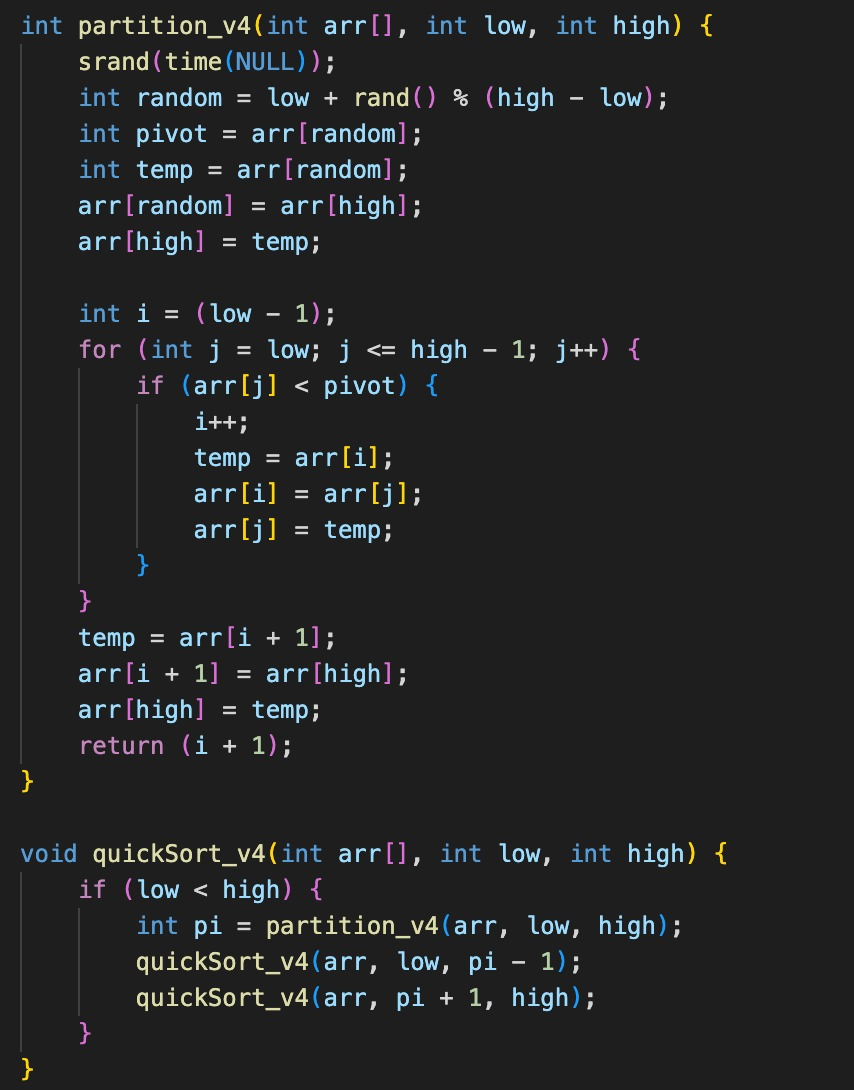
\includegraphics[width = 10cm]{Imagens/Quick Sort/quick4.jpeg}
    \caption{Quick Sort 4}
    \label{grafico_insert}
\end{figure}
Nesta abordagem, o pivô é escolhido de forma aleatória. Esta estratégia ajuda a garantir que, em média, o array seja dividido de forma relativamente equilibrada, reduzindo a probabilidade de pior caso independente da ordenação inicial do array. A escolha aleatória é particularmente útil para evitar o pior caso em arrays que possam ter alguma ordem específica ou padrão.